\documentclass[10pt,a4paper,landscape]{article}
\usepackage[margin=12mm]{geometry}
\usepackage{amsmath}
\usepackage{graphicx}
\usepackage{tikz}
\usetikzlibrary{arrows.meta,calc}
\pagestyle{empty}
\setlength{\parindent}{0pt}

\begin{document}
\begin{center}
{\Large\bfseries ZMP-Based Stability Cost: Block Diagram}
\medskip

\[
u=\begin{bmatrix}a_{\mathrm{ref}}&\tau_A^T&\tau_{W,\mathrm{ref}}^T\end{bmatrix}^{T}
\]
Lift extension target (m) $\;|\;$ Arm joint torque (Nm)
$\;|\;$ Wheel torque commands (Nm)
\medskip

\resizebox{0.98\linewidth}{!}{%
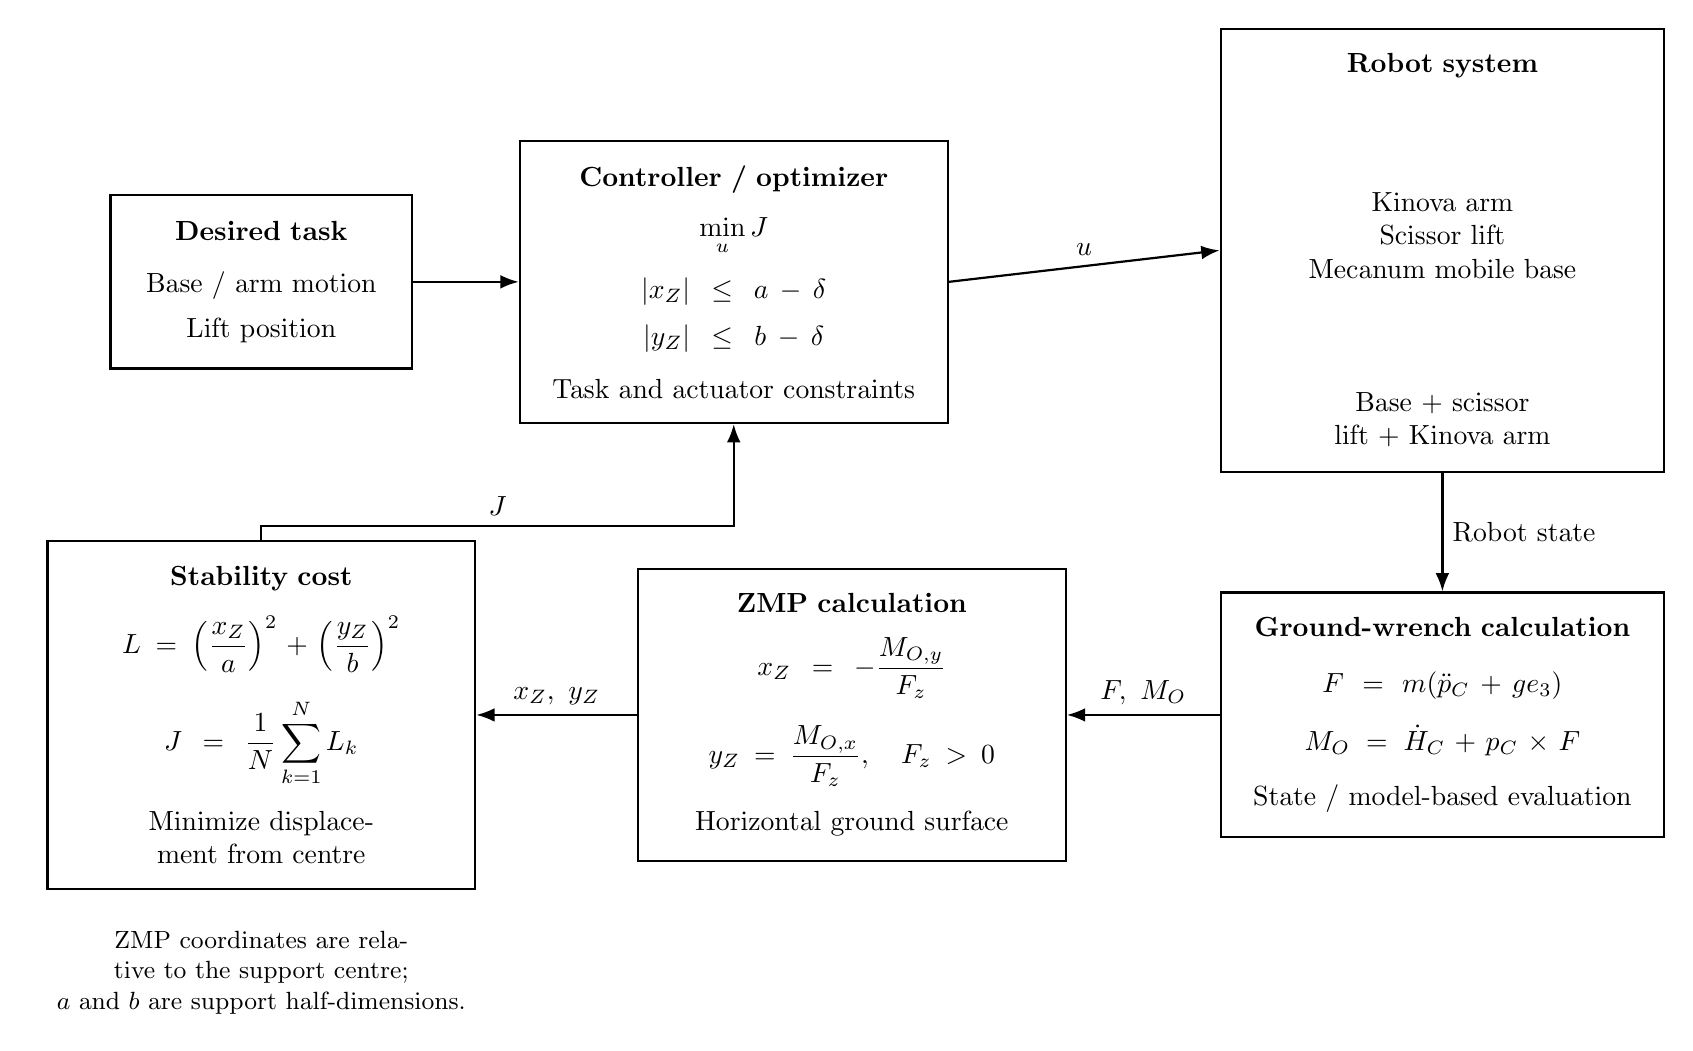
\begin{tikzpicture}[
  >=Latex,
  block/.style={draw,thick,rectangle,align=center,inner sep=9pt,font=\normalsize},
  signal/.style={->,thick},
  label/.style={font=\normalsize,align=center}
]

\node[block,text width=3.2cm,minimum height=2.2cm] (task) at (0,0)
  {\textbf{Desired task}\\[7pt]Base / arm motion\\[4pt]Lift position};

\node[block,text width=4.8cm,minimum height=3.5cm] (controller) at (6,0)
  {\textbf{Controller / optimizer}\\[6pt]
   $\displaystyle\min_u J$\\[7pt]
   $|x_Z|\le a-\delta$\\[5pt]
   $|y_Z|\le b-\delta$\\[7pt]
   Task and actuator constraints};

\node[block,text width=5cm,minimum height=5cm] (robot) at (15,0.4)
  {\textbf{Robot system}\\[6pt]
   % Keep robot_reference.png next to this file to show your robot image.
   % The fallback permits compilation in single-file editors.
   \IfFileExists{robot_reference.png}{%
     \includegraphics[height=3.5cm]{robot_reference.png}%
   }{%
     \parbox[c][3.5cm][c]{4cm}{\centering Kinova arm\\Scissor lift\\Mecanum mobile base}%
   }\\[6pt]
   Base + scissor lift + Kinova arm};

\node[block,text width=5cm,minimum height=2.8cm] (wrench) at (15,-5.5)
  {\textbf{Ground-wrench calculation}\\[8pt]
   $\displaystyle F=m(\ddot p_C+ge_3)$\\[9pt]
   $\displaystyle M_O=\dot H_C+p_C\times F$\\[8pt]
   State / model-based evaluation};

\node[block,text width=4.8cm,minimum height=2.8cm] (zmp) at (7.5,-5.5)
  {\textbf{ZMP calculation}\\[8pt]
   $\displaystyle x_Z=-\frac{M_{O,y}}{F_z}$\\[9pt]
   $\displaystyle y_Z=\frac{M_{O,x}}{F_z},\quad F_z>0$\\[8pt]
   Horizontal ground surface};

\node[block,text width=4.8cm,minimum height=2.8cm] (cost) at (0,-5.5)
  {\textbf{Stability cost}\\[8pt]
   $\displaystyle L=\left(\frac{x_Z}{a}\right)^2+
                       \left(\frac{y_Z}{b}\right)^2$\\[9pt]
   $\displaystyle J=\frac1N\sum_{k=1}^{N}L_k$\\[8pt]
   Minimize displacement from centre};

\draw[signal] (task.east)--(controller.west);
\draw[signal] (controller.east)--node[label,above] {$u$}(robot.west);
\draw[signal] (robot.south)--node[label,right] {Robot state}(wrench.north);
\draw[signal] (wrench.west)--node[label,above] {$F,\ M_O$}(zmp.east);
\draw[signal] (zmp.west)--node[label,above] {$x_Z,\ y_Z$}(cost.east);
\draw[signal] (cost.north)--(0,-3.1)--node[label,above] {$J$}
  (6,-3.1)--(controller.south);

\node[align=center,font=\small,anchor=north,text width=5.7cm]
  at ([yshift=-4mm]cost.south)
  {ZMP coordinates are relative to the support centre;\\
   $a$ and $b$ are support half-dimensions.};

\end{tikzpicture}%
}
\end{center}
\end{document}
